\documentclass[8pt,t,usepdftitle=false]{beamer}
\usetheme{Juelich}
\usepackage{setspace}
\usepackage[official]{eurosym}
\usepackage{bm}
\usepackage{mathtools}
%\usepackage{enumitem}\setitemize{itemsep=1ex}
\usepackage[%
backend=bibtex,
style=authoryear,
doi=true,
isbn=true,
url=true,
eprint=false,
sorting=nyt]{biblatex}
\addbibresource{refs.bib}
\usepackage{listings}
\lstset{
    basicstyle=\footnotesize,
    commentstyle=\color{blue},
    stringstyle=\sffamily,
    texcl=false,
    numbers=left,
    numberstyle=\tiny,
    stepnumber=1,
    numbersep=2ex,
    showstringspaces=false,
    captionpos=b,
    lineskip=0ex,%1pt,
    aboveskip=10pt,
    belowskip=10pt,
    frame=tb,
    showlines=true
}

\fzjset{
  title=regular,
  subtitle=regular,
  part=regular,
}

\setbeamerfont{title}{size*={10pt}{10pt},series=\bfseries}
\setbeamerfont{subtitle}{size*={12pt}{12pt},series=\bfseries\color{white}}
\setbeamerfont{frametitle}{size*={14pt}{14pt},series=\bfseries}
\setbeamertemplate{navigation symbols}{}

\setbeamertemplate{itemize/enumerate body begin}{\normalsize}
\setbeamertemplate{itemize/enumerate subbody begin}{\normalsize}
\setbeamertemplate{itemize/enumerate subsubbody begin}{\normalsize}
\setbeamertemplate{itemize/enumerate subsubsubbody begin}{\normalsize}

\mode<presentation>
{
  \usetheme{default}
  %% \setbeamercovered{transparent}
  \usefonttheme{professionalfonts}
  \usefonttheme{structurebold}
  \usecolortheme[rgb={0,0.3,0.6}]{structure}
}

% Delete this, if you do not want the table of contents to pop up at
% the beginning of each subsection:
% \AtBeginSection[]
% {
%   %\begin{frame}<beamer>
%     \begin{frame}[plain]
%     \frametitle{Outline}
%     \tableofcontents[currentsection]
%   \end{frame}
% }

\setlength{\leftmarginii}{3ex}

\setbeamercolor{alerted text}{fg=fzjblue}

\renewcommand{\arraystretch}{1.5}

\hypersetup{colorlinks,linkcolor=fzjblue,urlcolor=fzjblue,citecolor=fzjblue}

\newcommand{\Ex}{\text{E}}
\newcommand{\In}{\text{I}}
\newcommand{\inp}{\text{inp}}
\newcommand{\rest}{\text{rest}}
\newcommand{\tauM}{\tau_{\text{m}}}
\newcommand{\tauR}{\tau_{\text{ref}}{}}
\newcommand{\tauS}{\tau_{\text{S}}{}}

%%%%%%%%%%%%%%%%%%%%%%%%%%%%%%%%%%%%%%%%%%%%%%%%%%%%%%%%%%%%%%%%%%%%%%%%%%%%%%%%%%%%%%%%%%%%%%%%%
%% macros
\def\figpath{./figures}

\hypersetup{
  pdftitle={Introduction to NESTML},
  pdfauthor={Tom Tetzlaff}
  }

%%%%%%%%%%%%%%%%%%%%%%%%%%%%%%%%%%%%%%%%%%%%%%%%%%%%%%%%%%%%%%%%%%%%%%%%%%%%%%%%%%
\title{%
  {\LARGE\bf Introduction to NESTML}
  \hfill
\includegraphics[width=0.15\linewidth]{./figures/nestml-logo}\\[1ex]
}
\subtitle{%
  {\normalsize\mdseries Tom Tetzlaff}%
  %{\hfill\tiny\url{t.tetzlaff{at}fz-juelich.de}}\\
  {\hfill\tiny\texttt{t.tetzlaff@fz-juelich.de}}\\  
  {\footnotesize\mdseries Institute of Neuroscience and Medicine (INM-6), J\"ulich Research Centre and JARA}
  %{\hfill\tiny\url{http://www.csn.fz-juelich.de}}
  {\hfill\tiny\texttt{http://www.csn.fz-juelich.de}}
  \\
  {\tiny\mdseries EITN fall school, Paris, 22.09.2023}
  {\hfill\tiny\texttt{https://github.com/tomtetzlaff/2023\_eitnfallschool}}
}
\date{}
\author{}
\institute{}

%%%%%%%%%%%%%%%%%%%%%%%%%%%%%%%%%%%%%%%%%%%%%%%%%%%%%%%%%%%%%%%%%%%%%%%%%%%%%%%%%%%%%%%%%%%%%%%%%
\begin{document}
\maketitle

%%%%%%%%%%%%%%%%%%%%%%%%%%%%%%%%%%%%%%%%%%%%%%%%%%%%%%%%%%%%%%%%%%%%%%%%%%%%%%%%%%%%%%%%%%%%%%%%%
\begin{frame}[plain]
  \begin{center}
    \parbox{0.9\linewidth}{
      \vspace{0.95\textheight}
      \parbox[c]{0.1\linewidth}{%
        \href{https://creativecommons.org/licenses/by-sa/4.0}{%
          
\includegraphics[width=\linewidth]{\figpath/by-sa.png}}}
      \parbox[c]{0.9\linewidth}{\scriptsize%
        ~~{}This presentation is provided under the terms of the Creative Commons Attribution-ShareAlike License 4.0.
      }
    }    
  \end{center}
\end{frame}
%%%%%%%%%%%%%%%%%%%%%%%%%%%%%%%%%%%%%%%%%%%%%%%%%%%%%%%%%%%%%%%%%%%%%%%%%%%%%%%%%%%%%%%%%%%%%%%%%
\def\ttl{Outline}
\pdfbookmark[2]{Outline}{Outline}
\begin{frame}[plain]
  \frametitle{\ttl}
  \tableofcontents
\end{frame}
%%%%%%%%%%%%%%%%%%%%%%%%%%%%%%%%%%%%%%%%%%%%%%%%%%%%%%%%%%%%%%%%%%%%%%%%%%%%%%%%%%%%%%%%%%%%%%%%%
\def\ttl{Overview}\section{\ttl}
\begin{frame}[t,plain]
  \frametitle{\ttl}
  \begin{itemize}
  \item domain-specific language for definition of \emph{custom neuron and synapse models}
  \item specifically tailored for NEST (SpiNNaker and \href{https://nest-gpu.readthedocs.io}{NEST GPU} support in progress)
  \item NESTML toolchain includes
    \begin{itemize}
    \item syntax validation
    \item system analysis and automatized selection of appropriate solving method (using \href{https://ode-toolbox.readthedocs.io}{ODE-toolbox})
    \item code generation (C++ for NEST)
    \end{itemize}
  \item see \href{https://nestml.readthedocs.io/en/latest/nestml_language/nestml_language_concepts.html}{NESTML language concepts}\\[2ex]
    \begin{center}      
      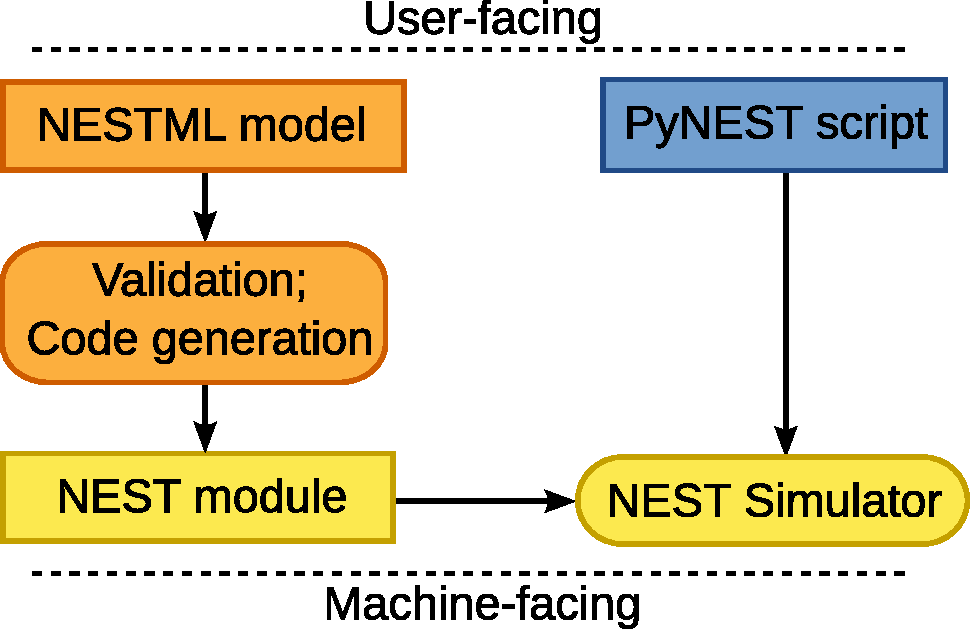
\includegraphics[width=0.5\linewidth]{./figures/nestml-workflow.pdf}
    \end{center}
    \vspace*{2ex}
  \item code: \url{https://github.com/nest/nestml}
  \item docs: \url{https://nestml.readthedocs.io}
  \item[] \vspace*{-5ex}\hfill
\includegraphics[width=0.2\linewidth]{./figures/nestml-logo.pdf}
  \end{itemize}
\end{frame}

%%%%%%%%%%%%%%%%%%%%%%%%%%%%%%%%%%%%%%%%%%%%%%%%%%%%%%%%%%%%%%%%%%%%%%%%%%%%%%%%%%%%%%%%%%%%%%%%%
\def\ttl{``Hello world (neuron)!''}\section{\ttl}
\begin{frame}[t,plain,allowframebreaks]
  \frametitle{\ttl}
  \frametitle{\ttl: NESTML model definition}
  \vspace*{-1ex}    
  \lstinputlisting
  [firstnumber=auto,name=helloworldnestml,showstringspaces=false,linerange={42-96}]
  {../code/nestml/iaf_psc_exp.nestml}
  %%
  \vspace*{-2ex}{\tiny (see \texttt{iaf\_psc\_exp.nestml})}
\end{frame}
%%%%%%%%%%%%%%%%%%%%%%%%%%%%%%%%%%%%%%%%%
\begin{frame}[t,plain]  
  \frametitle{\ttl: PyNEST code}
  \onslide<1->{
    \rule{\linewidth}{0.5pt}\\[-1ex]
    %%%
    \lstinputlisting
    [firstnumber=auto,language=Python,name=helloworldnestml,showstringspaces=false,linerange={1-16},frame=none]
    {../code/pynest/hello_world_nestml.py}
    %%
    \ldots\\
    %%
    \lstinputlisting
    [firstnumber=40,language=Python,name=helloworldnestml,showstringspaces=false,linerange={40-41},frame=none]
    {../code/pynest/hello_world_nestml.py}
    %%%
    \vspace*{-1ex}    
    \rule{\linewidth}{0.5pt}
    %% 
    \vspace*{-2ex}{\tiny (see \texttt{hello\_world\_nestml.py})}\\
  }
  \onslide<2->{
    \vspace*{-2.1cm}
    \hspace*{\fill}
    \fcolorbox{black}{white}{\parbox{0.4\linewidth}{
        \footnotesize
        \texttt{hello\_world\_nestml.pdf}:\\
        \includegraphics[width=\linewidth]{../code/pynest/figures/hello_world_nestml.pdf}
      }}
  }
\end{frame}
%%%%%%%%%%%%%%%%%%%%%%%%%%%%%%%%%%%%%%%%%%%%%%%%%%%%%%%%%%%%%%%%%%%%%%%%%%%%%%%%%%%%%%%%%%%%%%%%%
\def\ttl{``Hello world (synapse)!''}\section{\ttl}
\begin{frame}[t,plain]
  \frametitle{\ttl}
\end{frame}

%%%%%%%%%%%%%%%%%%%%%%%%%%%%%%%%%%%%%%%%%%%%%%%%%%%%%%%%%%%%%%%%%%%%%%%%%%%%%%%%%%%%%%%%%%%%%%%%% 
%%%%%%%%%%%%%%%%%%%%%%%%%%%%%%%%%%%%%%%%%%%%%%%%%%%%%%%%%%%%%%%%%%%%%%%%%%%%%%%%%%%%%%%%%%%%%%%%%
\begin{frame}[t,plain,allowframebreaks]
  \begin{center}
    \vspace*{\fill}
    \LARGE\emph{\it Thanks}
    \vspace*{\fill}
  \end{center}
\end{frame}
%%%%%%%%%%%%%%%%%%%%%%%%%%%%%%%%%%%%%%%%%%%%%%%%%%%%%%%%%%%%%%%%%%%%%%%%%%%%%%%%%%%%%%%%%%%%%%%%%
%% references
\setbeamertemplate{bibliography item}{}  %% remove document icon
\def\ttl{References}\section*{\ttl}
\begin{frame}[t,plain,allowframebreaks]  
  \frametitle{\ttl}
  \bibitemsep1ex
  \renewcommand{\bibfont}{\normalfont\small}
  \printbibliography
\end{frame}
%%%%%%%%%%%%%%%%%%%%%%%%%%%%%%%%%%%%%%%%%%%%%%%%%%%%%%%%%%%%%%%%%%%%%%%%%%%%%%%%%%%%%%%%%%%%%%%%%
\end{document}
%%%%%%%%%%%%%%%%%%%%%%%%%%%%%%%%%%%%%%%%%%%%%%%%%%%%%%%%%%%%%%%%%%%%%%%%%%%%%%%%%%%%%%%%%%%%%%%%%
%%%%%%%%%%%%%%%%%%%%%%%%%%%%%%%%%%%%%%%%%%%%%%%%%%%%%%%%%%%%%%%%%%%%%%%%%%%%%%%%%%%%%%%%%%%%%%%%%

%%% Local Variables:
%%% mode: latex
%%% TeX-master: t
%%% End:
